\documentclass[12pt]{article}

\usepackage[english]{babel}
\usepackage[utf8x]{inputenc}
\usepackage{amsmath}
\usepackage{graphicx}
\usepackage[colorinlistoftodos]{todonotes}
\usepackage{listings}
\usepackage{color}
\usepackage{indentfirst}

\definecolor{nGreen}{rgb}{0,0.6,0}
\definecolor{nGray}{rgb}{0.5,0.5,0.5}
\definecolor{nPurple}{rgb}{0.58,0,0.82}
\lstset{ 
  backgroundcolor=\color{white},   
  basicstyle=\footnotesize,       
  breakatwhitespace=false,         
  breaklines=true,                
  captionpos=b,                  
  commentstyle=\color{nGreen},   
  extendedchars=true,             
  frame=false,	                 
  keepspaces=true,                 
  keywordstyle=\color{blue},                  
  numbers=left,                   
  numbersep=5pt,                  
  numberstyle=\tiny\color{nGray}, 
  rulecolor=\color{black},        
  showspaces=false,               
  showstringspaces=false,         
  showtabs=false,                 
  stepnumber=1,                   
  stringstyle=\color{nPurple},    
  tabsize=2,	                  
  title=\lstname                  
}

\title{Relational DataBase}
\author{Arturo Chinchilla Sánchez, Malcolm Davis Steele}
\begin{document}
\maketitle
%------------------------------------------------------------------------------------------
% 	ABSTRACT
%------------------------------------------------------------------------------------------
\begin{abstract}
There are several paradigms of programming, object-oriented paradigm, Imperative, functional, logical, etc. For purposes of this project, is be used the functional programming paradigm, in conjunction with the Racket programming language , which belongs to the family of Lisp, as a functional language that it is. The Functional Paradigm as it's name says, used functions for all the operations and integrates math functions for operate the data. 
Internet is currently used for multiple purposes, but one of the primary, and which any Internet user is saved, is to do a search on your favorite search engine, search for the name of a song, the name of a plant, sound of an animal or to see that movies are on the undercard of film, from where we get this information? We obtain databases stored on Internet servers, to which we have access through the network. The databases contain information of all kinds, which are related to each other. A database can be from the list of employees of a company to a list of scientific names of trees.
But how programming paradigms relate to databases? the answer is very simle, databases are created using computer programs such as programming languages, which use paradigms, to carry out their tasks. So in this project we will create a relational database called "RELDB" using Racket and functional paradigm.
\end{abstract}
%----------------------------------------------------------------------------------------

%---------------------------------------------------------------------------------------
%	CONTENTS AND FIGURES
%---------------------------------------------------------------------------------------
\newpage
\tableofcontents % Prints the main table of contents
\listoffigures % Prints the list of figures

%----------------------------------------------------------------------------------------
%  INTRODUCTION
%-----------------------------------------------------------------------------------------
\newpage
\section{Introduction}

In computing the functional paradigm is a declarative programming paradigm, based on the use of functions, which are first-class citizens, which go hand in hand with recursion. This paradigm has it's beginnings in the simplest programming language, "The Lambda Calculus" which was a system developed in the 1930s for research and application of functions and recursion. Various programming languages are based in this paradigm, such as Lisp, Scheme, Erlang, Rust, Objective Caml, Scala, F \# and Haskell. Although the functional paradigm consists only of definitions of functions, actually, many programming languages that use this paradigm, have implemented functions that don't belong to the paradigm, which are called impure functions, and therefore are also called impure languages that incorporates these.
\newline
Racket is a programming language, which belongs to the large family of Lisp, although it is multi-paradigm, it is generally used in the functional paradigm. Developed in 1994 by PLT Inc. as an pedagogic programming environment based on Scheme, and MrEd, the first virtual machine for Racket was created. Later they developed DrScheme with PLT Scheme as the primary development language. Racket is very flexible, even without the use of dialects. Features such as the use of macros, tail recursion, and much more, allow it to be used to perform all kinds of tasks, from generation graphics web scrapers. Additionally, the powerful macro system allows developers to control all aspects of a language, which was one of the main goals behind it's design.
\newline
A database is a collection of information containing information on various topics, and they are categorized in different ways, but they are related to each other. All these data are stored for later use. If we see it in this way, a library can be considered a database. Today with the intensive use of electronic devices such as computers, smart phones, etc, besides the Internet, have been created thousands of digital databases, and have been stored on servers which are accessed via the web, for ensure that information reaches more people and of a faster way.
\newpage

%------------------------------------------------------------------------------------------
% USER GUIDE
%------------------------------------------------------------------------------------------
\section{User Guide}
\subsection{Software and Hardware Requirements}
\begin{itemize}
\item Operating System: OS based on Linux (Recommend Linuz Mint 17.2)
\item CPU: Intel Dual Core at 2GHz or equivalent
\item RAM Memory: 2GB (Recommend 4 or more) 
\item DrRacket IDE installed

\subsection{How to use:}
For the Data Base use the following commands:
\begin{itemize}
\item addt or addtable for add tables in the Data Base. Example:\newline
addt Person ID Name LastName\newline
addtable Person ID Name LastName\newline
When ID it's the Primary key. Take care, if you don't entry the Primary key the program don't allow you to insert the table.See Fig \ref{addt}
\begin{figure}[h!]
 	\centering
  	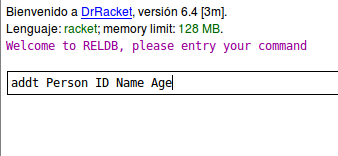
\includegraphics[scale=0.5]
  	{Images/1.png}
  	\caption{Example addt.}
     \label{addt}
\end{figure}
\item ins or insert for insert registers into a table. Example: \newline 
ins Person 12345 Dereck Molloy \newline
insert Person 12345 Dereck Molloy \newline
Then the command you give the table name that you want to insert the data. Take care, if you don't give the correct data, the program don't allow you to insert the registers. See Fig \ref{ins}
\begin{figure}[h!]
 	\centering
  	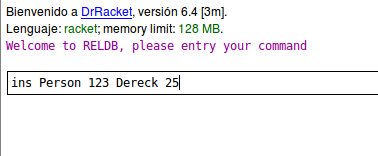
\includegraphics[scale=0.5]
  	{Images/2.png}
  	\caption{Example ins.}
     \label{ins}
\end{figure}

\item addr or addReference for create references.\newline
addr Car Owner Person \newline
addReference Car Owner Person \newline
Note that both tables should exist.See Fig \ref{addr}
\begin{figure}[h!]
 	\centering
  	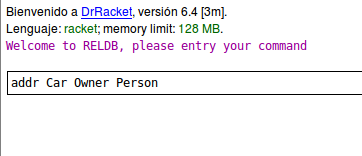
\includegraphics[scale=0.5]
  	{Images/3.png}
  	\caption{Example addr.}
     \label{addr}
\end{figure}
\item remr or removeReference for remove the reference. \newline
remr Car Owner Person \newline
removeReference Car Owner Person \newline
The reference should exist for be removed.
\item rr or remover to remove registers of the table\newline
rr Person 12345\newline
remover Person 12345\newline
You should indicate the table name and the Primary key.
\end{itemize}

\section{Development environment}
\subsection{DrRacket}
The Racket platform provide the "DrRacket" tool, which it's an Integrated Development Environment, programmed in Racket language, which will facilitate the task of programming in Racket. It also offers raco a tool for command line that will allow us to install packages or compile libraries. See Fig \ref{racket}

\begin{figure}[h!]
 	\centering
  	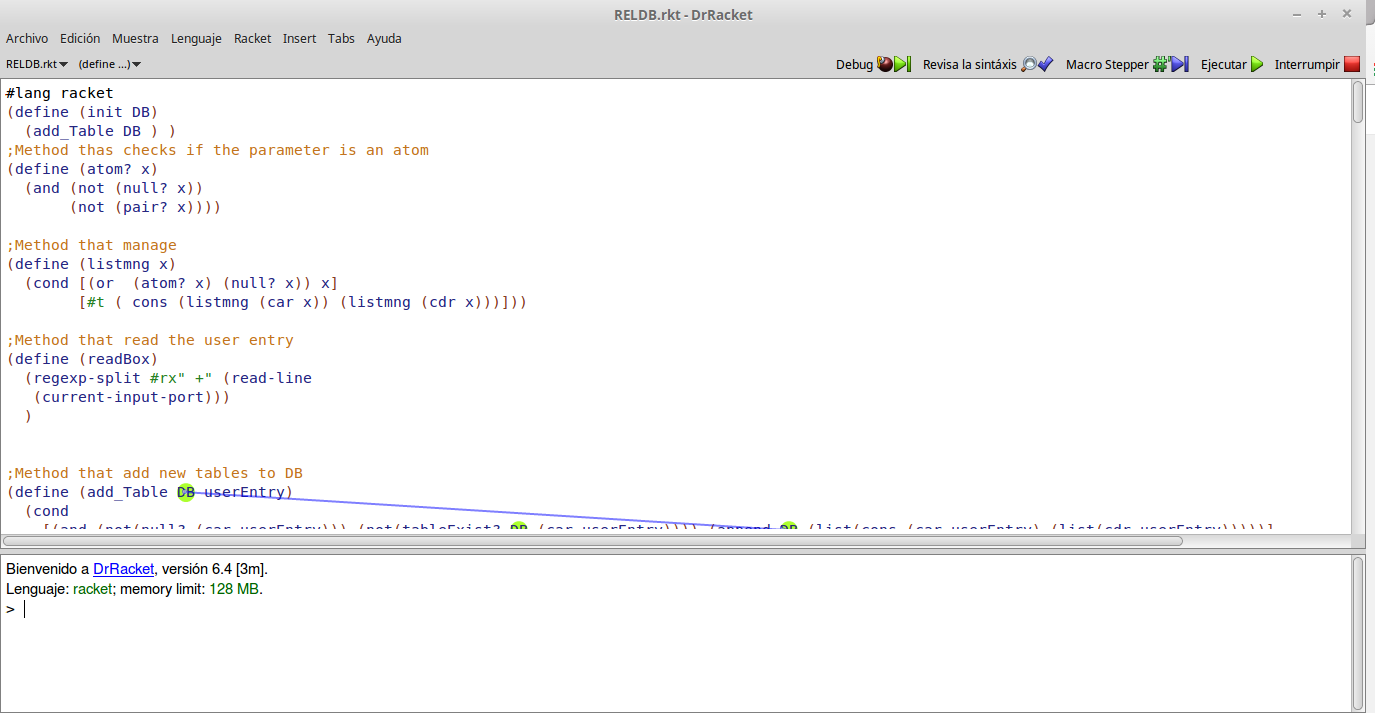
\includegraphics[scale=0.3]
  	{Images/drracket.png}
  	\caption{DrRacket Interface.}
     \label{racket}
\end{figure}
\subsection{Git and Github}
To store the code in a practical way and have a versioning control Git is used  for creating repositories and GitHub as service and cloud storage. This code manager (Git) let us to create branches for each member of the group and work separately, change the branch work, see and edit code of another branches, make commits for later if you want to go back in your code and when each part needed is done they can be merged into master branch to have a final version of the code. See Fig \ref{git}
\begin{figure}[h!]
 	\centering
  	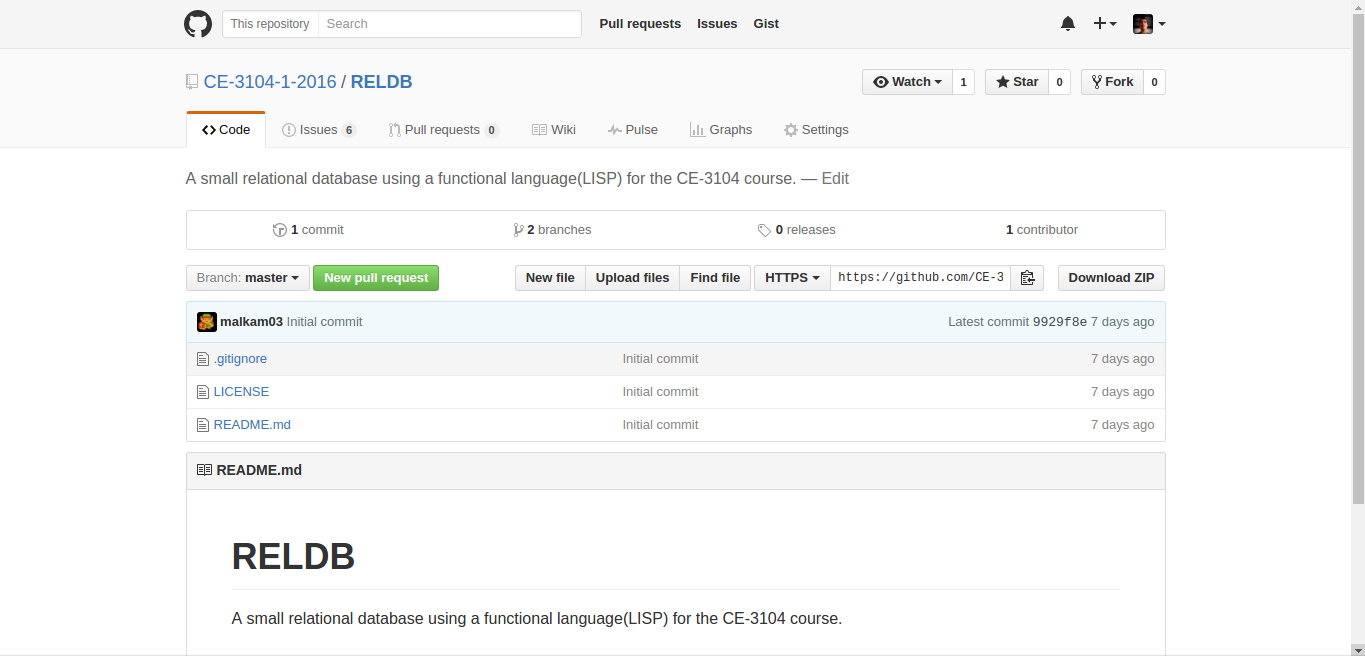
\includegraphics[scale=0.3]
  	{Images/GIT.png}
  	\caption{GitHub Interface.}
     \label{git}
\end{figure}

\subsection{Zube.io}
Zube is a free online service that provides the ability to organize, divide and manage a number of tasks by using a board, in addition to divide tasks by individual, organized by tasks remaining to be done, in process and finished . besides being able to put delivery dates and stages of the project. One of the possibilities Zube offers is the ability to connect to GitHub. See fig \ref{zube}
\begin{figure}[h!]
 	\centering
  	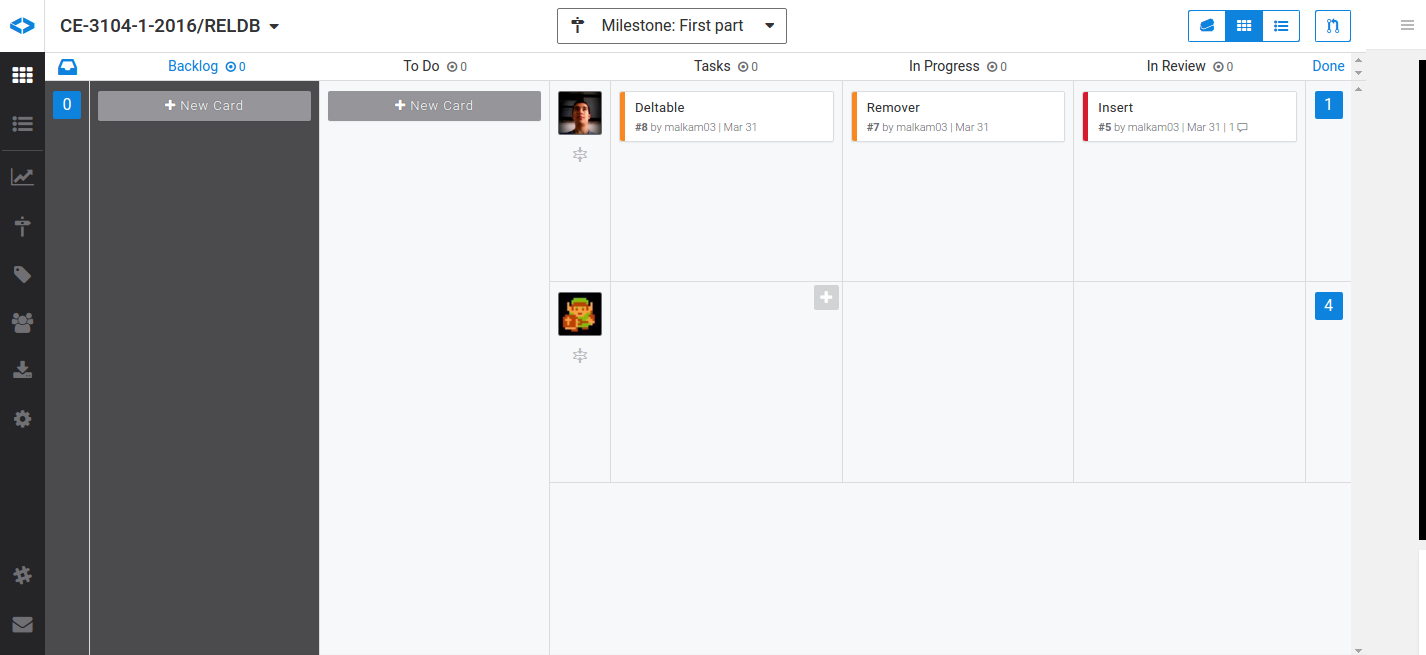
\includegraphics[scale=0.3]
  	{Images/zube.png}
  	\caption{Zube Dashboard.}
     \label{zube}
\end{figure}

\subsection{Codeshare.io}
CodeShare is a free online service that lets you share text in real time, but that is optimized for code sharing programming languages. This tool allows us to create a personalized web address (within your domain "https://codeshare.io/example") where anyone can enter, view and edit the shared material. It also has the option to create chats and video calls. It is a quick and easy way to share ideas and / or information with our workmates. See fig \ref{codeshare}
\begin{figure}[h!]
 	\centering
  	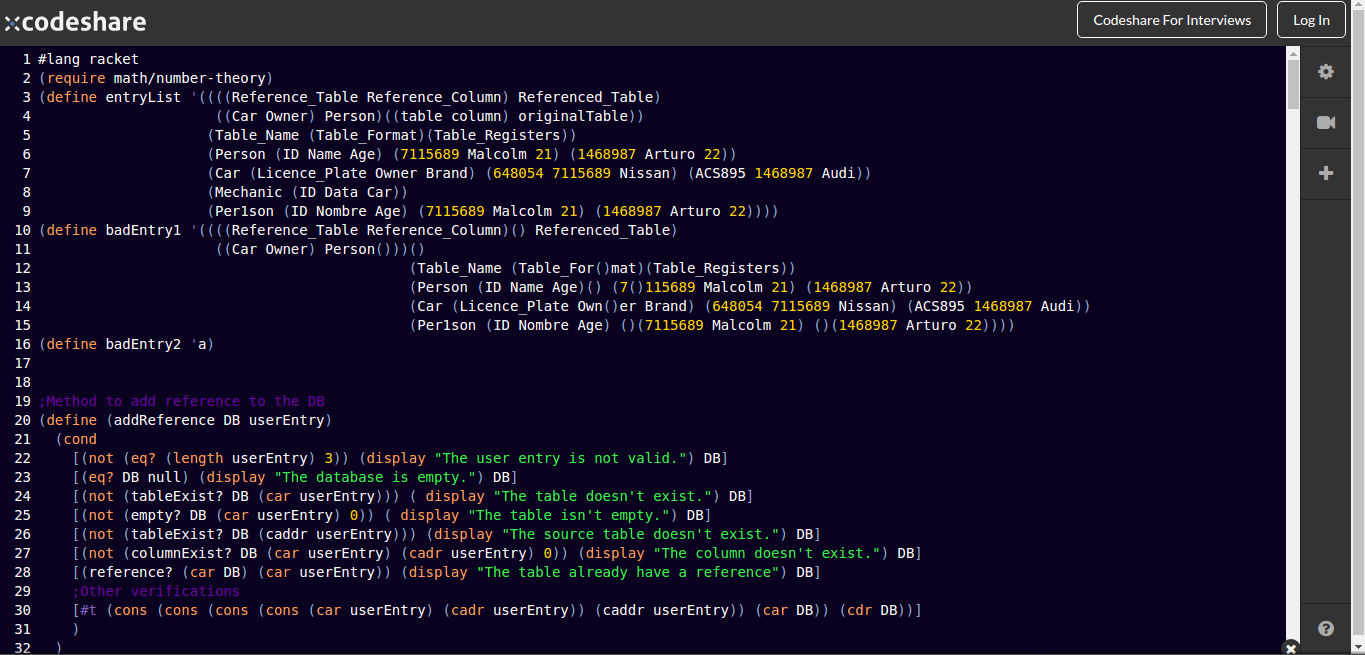
\includegraphics[scale=0.3]
  	{Images/CodeShare.png}
  	\caption{CodeShare Interfaces.}
     \label{codeshare}
\end{figure}

\subsection{Overleaf}
Free online tool used to write academic documents. This service allow create, edit and share your documents easily using \LaTeX. Provide two principal windows, in the first you can write your document, obviously using the \LaTeX syntax, and the second you can see your compiled document. \LaTeX also is composed of a large set of macros getting documents have a typographic high quality. Therefore it is widely used for the creation of academic papers, theses and technical books, since the typographic quality and made with \LaTeX documents is comparable to that of a great scientific publishing. See Fig \ref{overleaf}
\begin{figure}[h!]
 	\centering
  	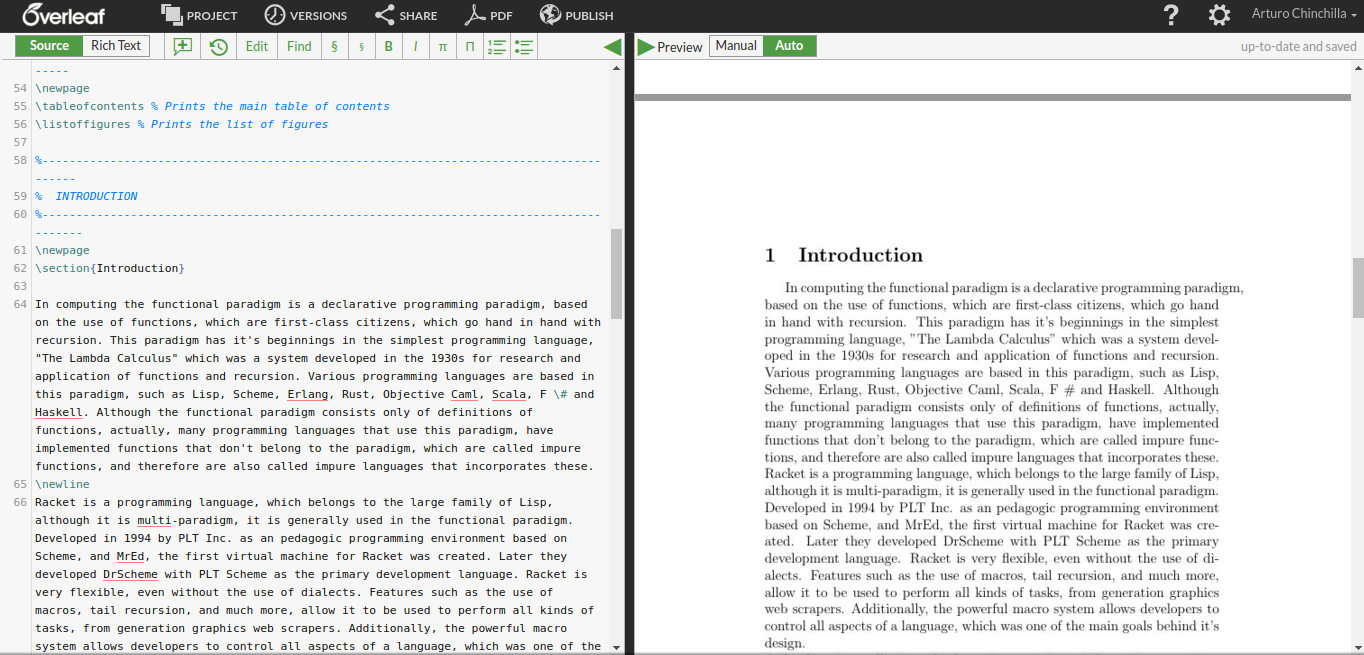
\includegraphics[scale=0.3]
  	{Images/overleaf.png}
  	\caption{Overleaf Interface Code-Compiled.}
     \label{overleaf}
\end{figure}


\section{Data Structures and functions}
\subsection{Lists}
The lists originally were the principal storage structures for programming languages that use the Functional Paradigm, like LISP or SCHEME, this while they were still completely pure, in fact Lisp is named for the acronym "LISt Processing".  Actually it's have been modified / adapted to give more flexibility to the programmer, introducing features that not belong to the functional paradigm, making impure the languages. Functions like the use of instantiated variables, the cycles “for” and “while”, etc.
\subsection{List Implementation.}
Since this project is about the functional paradigm, the list is the only data structure used because it could not use impure aspects of language. \newline
The database uses this list to store all the data that users enter, the implementation is a list of lists, where the first sub-list is a list of references and all other lists are tables with their respective parameters and records. An examples of such a lists would look like is shown.
\begin{enumerate}
\item A null list \newline
'[ ( ) ] \newline
The center list is the space for references
\item A list with tables but no references \newline
'[ ( ) (Table1 (Param1...Paramx) ) (Table2 (Param1...Paramx) ) ]\newline 
The references list is null, and the others tables are full.
\item A list with references and tables \newline
[((Table1 Paramx) Table2) (Table1 (Param1...Paramx)) (Table2 (Param1...Paramx))]\newline
When a the Parameterx of Table 1 makes reference to the Primary Key of the Table2.


\end{enumerate}


\section{Student activity log}
\subsection{Arturo's Time-Sheet}
\begin{center}
\begin{tabular}{ |c|c|c| } 
 \hline
 Date & Task Description & Spent Time \\ 
 \hline\hline
 04/02/2016 & Create a method that gets user entries and put it into a list. & 4 hours\\
 04/02/2016 & Create a method that creates lists(tables) into a list(DB) & 2 hours\\
 04/02/2016 & Create a method that insert registers without parameter & 6 hours\\
 04/02/2016 & Create method that manage the user entry by box entry  & 3 hours \\
 04/03/2016 & Fix the method add\_Table, adding the restrictions & 0.5 hours \\
 04/03/2016 & Create method that manage the insertions& 0.5 hours\\
 04/03/2016 & Create method that found a referenced table of a given table & 5 hours \\
 04/03/2016 & Create method that check if a register is in a table & 2 hours \\
 04/03/2016 & Fix the method mngIns & 1 hour \\
 04/05/2016 & Fix the method insert\_data for uncompleted or more registers & 2 hours \\
 04/06/2016 & Creating auxiliaries functions & 6 hours\\
 04/06/2016 & Fix some bugs (Voids elements) & 15 hours\\
 04/07/2016 & Making the external documentation & 12 hours\\
 

 \hline
 & Total & 59 hours\\ 
 \hline
\end{tabular}
\end{center}
\subsection{Malcolm's Time-Sheet} 
\begin{center}
\begin{tabular}{ |c|c|c|} 
 \hline
 Date &  Task Description &  Spent Time \\ 
 \hline\hline 
 04/02/2016 & Making the functions of add and remove references & 13 hours\\
 04/03/2016 & make auxiliaries functions for references & 13 hours \\
 04/04/2016 & Create the update method & 14 hours\\
 04/05/2016 & Fix some bugs for the program & 15 hours\\
 04/06/2016 & Create the method that show & 15 hours\\
 04/07/2016 & Create the methods of queries & 14 hours\\
 

  \hline
 & Total & 84 hours\\ 
 \hline
\end{tabular}
\end{center}
\section{Project final status}
Despite the nature of the project, and the amount of time this sued, because of the number of verifications, and the learning curve to a new programming language and a new paradigm, the project is accomplished almost entirely. Just leaving aside the storage processes.\newline\subsection{Issues, Limitations or Challenges}
\begin{itemize}
\item The large amount of verifications to be performed.
\item The implementation of REGEX for manage and split the users entries.
\item The learning curve of a new Programming Language and new Paradigm.
\item Make the update and query functions were a challenge, because it has a great difficult level.

\subsection{Known Issues}

\item Don't implemented the stored procedures.
\end{itemize}

\section{Conclusions, Suggestions and Recommendations}
\begin{itemize}
\item online tools can be helpful for remote work.
\item Tools like the handler code versions is very useful, because in case of any failure in the new version allows us to return to a previous, plus the possibility of linking it to the storage service in the cloud, to share, and work together in a very easy way.
\item Zube can be helpful for organize the tasks of the group.
\item The amount of verifications tha a Data Base have are exaggerated.
\item OverLeaf it's a very easy tool, for write papers and scientific papers.
\end{itemize}




\end{itemize}


%--------------------------------------------------------------------------------
%             References
%--------------------------------------------------------------------------------

\begin{thebibliography}{10}
\bibitem{Racket}

  \emph{"Welcome to Racket"}
   Docs.racket-lang.org, 
  2016 [Online]. 
 Available: http://docs.racket-lang.org/guide/intro.html. [Accessed: 08- Apr- 2016].
 
 \bibitem{Racket}
  \emph{"Racket Documentation"}
   Docs.racket-lang.org, 
  2016 [Online]. 
Available: https://docs.racket-lang.org/index.html. [Accessed: 08- Apr- 2016].
 \bibitem{Regex}
  \emph{"RegExr: Learn, Build, \& Test RegEx"}
   RegExr.com, 
2016. [Online]. Available: http://regexr.com/. [Accessed: 08- Apr- 2016]. 

\end{thebibliography}


\end{document}